% --------------------------------------------------------------
% This is all preamble stuff that you don't have to worry about.
% Head down to where it says "Start here"
% --------------------------------------------------------------
 
\documentclass[12pt]{article}
 
\usepackage[margin=1in]{geometry} 
\usepackage{amsmath,amsthm,amssymb}
\usepackage{listings}
\usepackage{enumitem}   
\usepackage{graphicx}
\graphicspath{ {./images/} }

\lstset{
   basicstyle=\fontsize{9}{10}\selectfont\ttfamily
}
 
\newcommand{\N}{\mathbb{N}}
\newcommand{\Z}{\mathbb{Z}}
 
\newenvironment{theorem}[2][Theorem]{\begin{trivlist}
\item[\hskip \labelsep {\bfseries #1}\hskip \labelsep {\bfseries #2.}]}{\end{trivlist}}
\newenvironment{lemma}[2][Lemma]{\begin{trivlist}
\item[\hskip \labelsep {\bfseries #1}\hskip \labelsep {\bfseries #2.}]}{\end{trivlist}}
\newenvironment{exercise}[2][Exercise]{\begin{trivlist}
\item[\hskip \labelsep {\bfseries #1}\hskip \labelsep {\bfseries #2.}]}{\end{trivlist}}
\newenvironment{reflection}[2][Reflection]{\begin{trivlist}
\item[\hskip \labelsep {\bfseries #1}\hskip \labelsep {\bfseries #2.}]}{\end{trivlist}}
\newenvironment{proposition}[2][Proposition]{\begin{trivlist}
\item[\hskip \labelsep {\bfseries #1}\hskip \labelsep {\bfseries #2.}]}{\end{trivlist}}
\newenvironment{corollary}[2][Corollary]{\begin{trivlist}
\item[\hskip \labelsep {\bfseries #1}\hskip \labelsep {\bfseries #2.}]}{\end{trivlist}}
 
\begin{document}
 
% --------------------------------------------------------------
%                         Start here
% --------------------------------------------------------------
 
%\renewcommand{\qedsymbol}{\filledbox}
 
\title{Homework 2}%replace X with the appropriate number
\author{Hai Nguyen \& Huan Nguyen\\ %replace with your name
STAT760 - Statistical Learning} %if necessary, replace with your course title
 
\maketitle
 
\textbf{Problem 1}
\\Train a multivariate regression predictor for lpsa using from one to eight predictors. Graph the training error for the eight possible regressions. Use all the data, without dividing into train \& test sets.

\begin{itemize}
\item Source code (Matlab):
\begin{lstlisting}[language=Matlab]
A = load('prostate.data');
Y = A(:,9);
error = zeros(8,1);
for i=1:8
    X = A(:,1:i);
    beta = inv(X'*X)*X'*Y;
    error(i) = (Y-X*beta)'*(Y-X*beta);
end
plot(error)
grid on
title('Training error of eight possible regression')
xlabel('Number of predictors')
ylabel('Training Error')
\end{lstlisting}
\item Output:

\begin{figure}[h!]
\begin{center}
  \caption{Graph the training error for the eight possible regressions}
  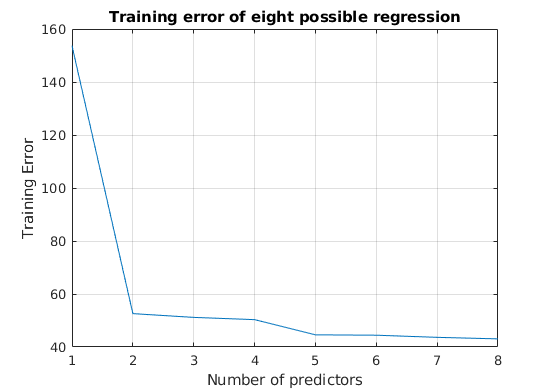
\includegraphics[width=0.5\textwidth]{images/hw2.png}
 \end{center}
\end{figure}

\item Comment:
Training error reduces when the number of predictors increases as the model is more complex. When the number of predictors is larger than 5, training error doesn't change much.   

\end{itemize}
\textbf{Problem 2}

\begin{enumerate}
    \item Suppose we have a data set with five predictors, $X_1 = \text{GPA}$, $X_2 = \text{IQ}, X_3 =\text{Gender}$ (1 for Female and 0 for Male), $X_4 =$ Interaction between GPA and IQ, and $X_5=$ Interaction between GPA and Gender. The response is starting salary after graduation (in thousands of dollars). Suppose we use least square to fit the model, and get $\hat{\beta}_0=50$, $\hat{\beta}_1=20$, $\hat{\beta}_0=0.07$, $\hat{\beta}_3=35$, $\hat{\beta}_4=0.01$, $\hat{\beta}_5=-10$.

\begin{enumerate}[label=(\alph*)]
    \item Which answer is correct, and why:
    
    \begin{enumerate}[label=(\roman*)]
        \item For a fixed value of IQ and GPA, males earn more on average than females.
        \item For a fixed value of IQ and GPA, females earn more on average than males.
        \item For a fixed value of IQ and GPA, males earn more on average than females provided that the GPA is high enough.
        \item For a fixed value of IQ and GPA, females earn more on average than males provided that the GPA is high enough.
        \\ \textit{The salary is given by:}
        \\$S = 50 + 20\text{GPA}+0.07\text{IQ}+35\text{Gender} + 0.01\text{GPA}\times\text{IQ} - 10\text{GPA}\times\text{Gender}$
        
        \textit{For a fixed value of IQ and GPA: }
        \\$S_{male} - S_{female} = 10\times\text{GPA}-35$ \textit{therefore (iii) is correct, (iv) is wrong and there is not enough information to evaluate (i) and (ii).}
    \end{enumerate}
    
    \item Predict the salary of a female with IQ of 110 and a GPA of 4.0.
    \\\textit{Use the above equation to calculate, we have $S = 50 + 20\times4.0 + 0.07\times110 + 35\times1.0 + 0.01\times110\times4.0-10\times4.0\times1.0 = 137.1$. Therefore the predicted salary is 137100$\$$.}
    \item True or False: Since the coefficient for the GPA/IQ interaction term is very small, there is very little evidence of an interaction effect. Justify your answer.
    \\ \textit{False, because the small coefficient does not mean small interaction effect since there are units of the two variables. Moreover, the significance of an interaction is different from the magnitude of the interaction.}
\end{enumerate}

\item I collect a set of data ($n = 100$ observations) containing a single predictor and a quantitative response. I then fit a linear regression model to the data, as well as a separate cubic regression, i.e. $Y= \beta_0 + \beta_1X + \beta_2X^2 + \beta_3X^3 + \epsilon$.
\begin{enumerate}[label=(\alph*)]
    \item Suppose that the true relationship between X and Y is linear, i.e.$Y=\beta_0 + \beta_1X + \epsilon$. Consider the training residual sum of squares (RSS) for the linear regression, and also the training RSS for the cubic regression. Would we expect one to be lower than the other, would we expect them to be the same, or is there not enough information to tell? Justify your answer.
    \\ \textit{There is high chance that the RSS of the linear regression will be lower than for the cubic regression as the true relation between X and Y is linear. However, it is difficult to know for sure because the answer would also depend on the training data.}
    \item Answer (a) using test rather than training RSS.
    \\ \textit{The RSS in this case will depend on the test data, so we have not enough information to tell. However, a reasonable assumption is that the cubic regression might be prone to overfit and therefore RSS with the test data will be higher.}
    \item Suppose that the true relationship between X and Y is not linear, but we don’t know how far it is from linear. Consider the training RSS for the linear regression, and also the training RSS for the cubic regression. Would we expect one to be lower than the other, would we expect them to be the same, or is there not enough information to tell? Justify your answer.
    \\\textit{Cube regression has more flexibility therefore it should have lower training RSS that the linear regression. Polynomial regression in general can more closely follow training points which will reduce the training RSS.}
    \item Answer (c) using test rather than training RSS.
    \\ \textit{There is not enough information to tell which test RSS would be lower as we do not know how close it is to linear relationship or cubic relationship. If it is closer to linear than cubic, the linear regression test RSS could be lower than the cubic regression test RSS. Or, if it is closer to cubic than linear, the cubic regression test RSS could be lower than the linear regression test RSS. We simply do not know what level of flexibility will fit data better.}
\end{enumerate}

\end{enumerate}


 
% --------------------------------------------------------------
%     You don't have to mess with anything below this line.
% --------------------------------------------------------------
 
\end{document}